% Chapter 4

\chapter{HomeLive Management Platform} % Main chapter title

\label{Chapter4} % For referencing the chapter elsewhere, use \ref{Chapter4}

\lhead{Chapter 4. \emph{HomeLive Management Platform}} % This is for the header on each page - perhaps a shortened title

%----------------------------------------------------------------------------------------
In this chapter, the Homelive Management Platform structure will be introduced. The following \autoref{fig:Platform} shows an global view for CWMP. With TR-069 protocol, ACS can communicate and manage devices easily.
%http://orange-france.com.francetelecom.fr:81/ui_normandie/spip.php?article3304
\begin{figure}[htbp]
	\centering
		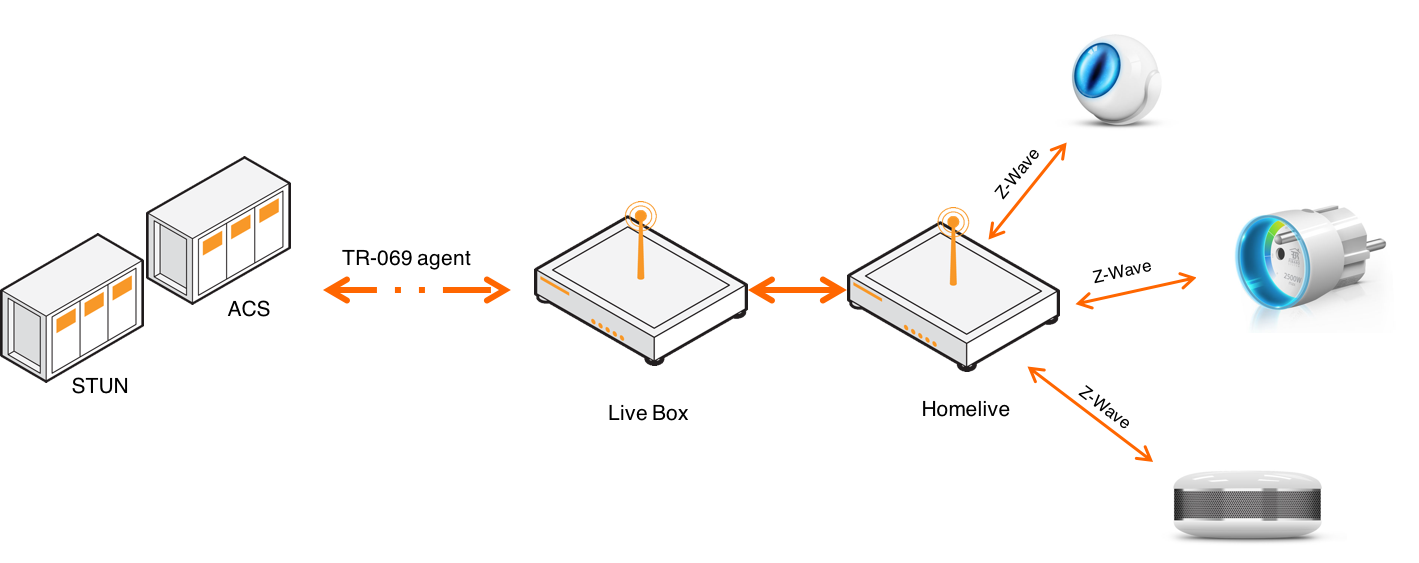
\includegraphics[width=9.5cm]{Figures/Homelive_Management_Platform.png}
	\caption[Homelive Management Platform]{Homelive Management Platform}
	\label{fig:Platform}
\end{figure}

ACS is the server which is accessible by the support engineers of Orange. Support engineers are capable to build a connection remotely with Homelive box using protocol TR-069. The connection are build by two programs. The \textit{TR-069 server} will be running in ACS as a server side and \textit{TR-069 client} will be running in Homelive as the client. This essentially means that control over the flow of the provisioning session is the sole responsibility of the device. Through TR-069, the high-level operations possible are:
\begin{itemize}
  \item Service activation and reconfiguration
  \begin{itemize}
    \item Initial configuration of the service as part of zero-touch or one-touch configuration process
    \item Service re-establishment (ex. after device is factory-reset, exchanged)
  \end{itemize}
  \item Remote Subscriber Support
  \begin{itemize}
    \item Verification of the device status and functionality
    \item Manual reconfiguration
  \end{itemize}
  \item Firmware and Configuration Management
  \begin{itemize}
    \item Firmware upgrade/downgrade
    \item Configuration backup/restore
  \end{itemize}
  \item Diagnostics and monitoring
  \begin{itemize}
    \item Throughput (TR-143) and connectivity diagnostics
    \item Parameter value retrieval
    \item Log file retrieval
  \end{itemize}
\end{itemize}
%----------------------------------------------------------------------------------------------------------------------
\section{Auto Configuration Server}
